\documentclass[12 pt]{article}
\usepackage[margin = 1cm]{geometry}
\usepackage [utf8]{inputenc}
\usepackage[T2A]{fontenc}
\usepackage[russian]{babel}
\usepackage{amsthm, amsmath, amssymb}
\usepackage{xcolor}
\definecolor{mygreen}{rgb}{0,0.6,0}
\usepackage{listings}
\usepackage{graphicx}
\usepackage{hyperref}
\lstset{
  language=Java,
  tabsize=2,
  belowcaptionskip=1\baselineskip,
  breaklines=true,
  xleftmargin=1cm,
  escapechar=|,
  showstringspaces=false,
  commentstyle=\color{green},
  keywordstyle=\color{blue},
  stringstyle=\color{mygreen},
  basicstyle=\footnotesize\ttfamily,
  numbers=left,
  commentstyle=\usefont{T2A}{fcr}{m}{sl}
}

\renewcommand{\O}{\mathcal{O}}
\newcommand{\SO}{\Rightarrow}
\newcommand{\EQ}{\Leftrightarrow}
\newcommand{\union}{\cup}
\renewcommand{\div}{\mathop{\raisebox{-2pt}{\vdots}}}

\begin{document}

\section{Android Manifest}
    \begin{itemize}
    	\item Описание проекта, в том числе настройки и конфигурации(например, версии).
    	\item Прописаны permission и составляющие проекта, такие как:
		\begin{enumerate}
        	\item Activity 
        	\item BroadCastReceiver 
        	\item Service
        \end{enumerate}
    \end{itemize}

\section{Activity}
    \begin{itemize}
    	\item Экран приложения
        \item Первой в программе вызывается Activity, к которому приходит интент MAIN. Это также прописывается в Android Manifest.
    	\item Цикл жизни:
   	\end{itemize}
	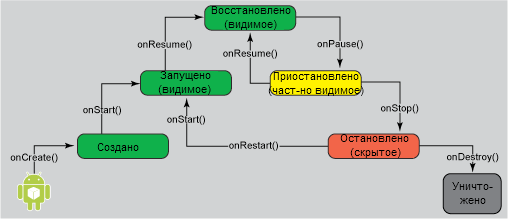
\includegraphics{LifeCycle.png}
    
\section{BroadCastReceiver} 
    
    BroadCastReceiver - класс-обработчик широковещательных сообщений(intent). Может быть подписан на несколько разных интентов. Если к нему приходит несколько интентов за раз, то они выстраиваются в цепочку и обрабатываются по одному, поэтому Android закрывает интент, если BroadCastReceiver пытается его обрабатывать больше положенного. Из-за этого количество действий, которое вы можете сделать с помощью BroadCastReceiver, довольно ограничено(обычное использование - послать другой интент, чтобы запустить Activity, Service или что-нибудь подобное).
    
    Другое назначение BroadCastReceiver это получать системные оповещения, такие как оповещения о маленьком заряде батарейки или о том, что Android загрузился.
    
    BroadCastReceiver региструется в Android Manifest'е так:
    \begin{lstlisting}
<receiver android:name=".LocationChangedReceiver" />
    \end{lstlisting} 
    
    В принципе, можно регистрировать и программно.
    
    Указать, на какие intent'ы подписан BroadCastReceiver, можно двумя способами:
	\begin{itemize}
    	\item В Android Manifest (обычно при подписке на системные события)
		\item Программно:
        \begin{lstlisting}
mLocationManager = (LocationManager)getSystemService(Context.LOCATION_SERVICE);
Intent intent = new Intent(this, LocationChangedReceiver.class);
mLocationChangedIntent =
PendingIntent.getBroadcast(this, 0, intent, PendingIntent.FLAG_UPDATE_CURRENT);
    \end{lstlisting}
    \end{itemize}
     Здесь:
	\begin{itemize}
    \item Получаем доступ к LocationManager
	\item Создаем Intent и прописываем класс, куда интент должен быть направлен.
	\item Рассылаем этот Intent, как широковещательное сообщение.
    \end{itemize}
	Класс Intent - это такой способ общаться между частями приложения. В него можно записать дополнительную информацию.
        \begin{lstlisting}
startService.putExtra(LocationManager.KEY_LOCATION_CHANGED, location);
        \end{lstlisting}        
        
    Доставать информацию из Intent можно так:
        \begin{lstlisting}
Location location = (Location) intent.getExtras().get(locationKey);
        \end{lstlisting}
    PendingIntent - наследник класса Intent. Главное его отличие от обычного интента в том, что он учитывает права приложения. Можно запускать Activity(приложение) из другого приложения, но у этого Activity(приложения) может не быть прав на работу с некоторыми ресурсами. Если эти права нужны, вы можете послать PendingIntent и передать тем самым Activity(приложению), которое вы запускаете, свои права на исполнение. Также некоторые API просто по умолчанию используют PendingIntent(например, так делает LocationManager). 
    
      Интенты бывают:
      \begin{itemize}
      		\item explicit - для них явно прописывается, к какому классу его отправить
            \item implicit - неявно описывается, куда нужно передать сообщение. Дальше в этом разбирается Android.
      \end{itemize}
      В коде выше интент - explicit. 
    
    Когда приходит интент, который предназначен для данного BroadCastReceiver, вызывается метод onReceive(). Одним из его аргументов является экземпляр класса Context - базовый класс для частей приложения. Через него можно обращаться к ресурсам Android. К примеру, Activity - наследник класса Context. Поэтому, мы можем вызвать, к примеру, метод getSystemService(), определённый в классе Context - для доступа к какому-то сервису. А вот BroadCastReceiver не является наследником класса Context, но доступ к различным менеджерам может понадобиться, поэтому контекст и передаётся методу onReceive(). 
    
        В нашем Receiver мы просто напечатаем в Log некое сообщение(что такое Log мы поподробнее ещё обсудим). 
        
        \begin{lstlisting}
public class LocationChangedReceiver extends BroadcastReceiver {

    private static final String TAG = LocationChangedReceiver.class.getSimpleName();

    public LocationChangedReceiver() { }

    @Override
    public void onReceive(Context context, Intent intent) {
        final String locationKey = LocationManager.KEY_LOCATION_CHANGED;

        if (intent.hasExtra(locationKey)) {
            Location location = (Location) intent.getExtras().get(locationKey);

            Intent startService = new Intent(context, ForecastUpdateService.class);
            startService.putExtra(LocationManager.KEY_LOCATION_CHANGED, location);
            context.startService(startService);
        }
    }
}
    \end{lstlisting}
    
    Если обобщить:
    \begin{itemize}
        \item Один из стандартных классов Android, завязан на несколько(может один) intent. 
	    \item Получает intent, к которому он привязан и \textcolor{red}{быстро} реагирует(с технической точки зрения при получении intent вызывается onReceive(), который должен быстро выполняться).
		\item Если один BroadCastReceiver соответствует нескольким intent, то они построятся в цепочку и будут выполняться последовательно.
		\item Поэтому если по какому-то intent метод выполняется слишком долго, то его выполнение оборвется, чтобы другие intent не ждали.
		\item Так что обычно, его используют только чтобы послать какой-то другой intent или получить системное оповещение.
 		\item Receiver должен быть прописан в Android Manifest.
        \begin{lstlisting}
<receiver android:name=".LocationChangedReceiver" />
        \end{lstlisting}		    
 	    \item Подписку на intent можно тоже записать в Manifest.
        \item А можно это сделать и програмно. Explicit intent - явно указываем класс, к которому intent отправить. Бывает ещё implicit intent.  
        \item Класс Context - это базовый класс для частей приложения. К примеру, Activity - наследник класса Context. Он предоставляет доступ ко всем андроидовским ресурсам и поэтому является параметром метода onReceive у BroadcastReceiver.
    \end{itemize}

\section{Log}     
    \begin{itemize}
        \item Записи в log выводятся на экран Device Monitor.Logcat.
        \item Логирование происходит так:
    \end{itemize}
    \begin{lstlisting}
    ...
private static final String TAG = 
            SMSReceiver.class.getSimpleName();
    ...
Log.d(TAG, "SMS received");    
    \end{lstlisting}

    \section{Service}    
    \begin{itemize}
        \item Service также надо прописывать в манифесете:
        \begin{lstlisting}
<service
    android:name=".DatabaseService"
    android:exported="false" >
</service>        
        \end{lstlisting}
        \item Для того, чтобы делать продолжительные действия BroadCastReceiver не подходит. Для этого нужно использовать Service.
        \item Ключ exported задаёт, позволено ли другим приложениям запускать наш сервис, Activity и тд.
        \item Если к нему обращаются много intent, они также становятся в очередь.
        \item Запускают intent к service через команду startService(...);
        \item При обработке intent запускается метод onHandleIntent(Intent intent);
    \end{itemize}
    
\section{Permissions}
    \begin{itemize}
        \item Чтобы работать с сетью надо подключить соотетсвующие permission.
        \begin{lstlisting}
<uses-permission android:name="android.permission.INTERNET" /> 
<uses-permission  android:name="android.permission.ACCESS_NETWORK_STATE"/>        
        \end{lstlisting}
    \end{itemize}
    
\section{Connection}
    \begin{itemize}
        \item Самый простой способ работать с сетью - это HttpURLConnection.
        \item Возвращается методом .openConnection():
        \begin{lstlisting}
URL url = new URL(uri.toString());
connection = 
        (HttpURLConnection) url.openConnection();
        \end{lstlisting}
        \item Протокол http может обрабатывать различные запросы. Например, запрос на получение информации. Если мы хотим получить информацию - пишем следующее:
        \begin{lstlisting}
connection.setRequestMethod("GET");
connection.connect();
        \end{lstlisting}
    \end{itemize}
    Пример считывания информации:
    \begin{lstlisting}
InputStream inputStream = connection.getInputStream();
StringBuilder buffer = new StringBuilder();
if (inputStream == null) {
    return;
}
reader = new BufferedReader(new InputStreamReader(inputStream));
String line;
while ((line = reader.readLine()) != null) {
    buffer.append(line);
    buffer.append("\n");
}

if (buffer.length() == 0) {
    return;
}
    \end{lstlisting}
        Обычно ответ формируется либо в формате xml, либо в формате json - это два разных представления данных. В данном случае, мы используем json. Нужно этот формат распарсить и обработать - для этого мы написали функцию parseJsonData(String), но подробно на ней останавливаться не будем.
    
    Каждый раз при смене своих координат не очень разумно слать запрос в интернет. Это долго, это не надёжно - интернет или сервис могут не работать. Поэтому стоит задуматься о том, как приложение будет работать в offline-режиме. К примеру, разумный вариант - когда у нас есть доступ к сети, получать погоду и сохранять её в базу данных. А когда сети нет - просто достаём из базы данных самое актуальное значение и показываем. Оно, может быть, и устаревшее, но хоть какое-то. Соответсвенно, следующая наша цель - получить результат и сохранить его в базу данных.
\section{Data bases}
	\begin{itemize}
		\item ContentProvider - это такой класс-обёртка над базой данных.
		\item Его также надо прописывать в манифесте:
		\begin{lstlisting}
<provider
	android:authorities="edu.spbau.android.forecast"
    android:name=".WeatherProvider" />		
		\end{lstlisting}
	\end{itemize}    
	Перд тем, как подробней говорить о ContentProvider, познакомимся с ещё одним классом Contract, реализация которого является правилом хорошего тона. Там обычно описывается структура базы данных. То есть, он необязателен, чтобы работать с базами данных, но лучше его реализовывать.
	Соответсвенно:
	\begin{itemize}
	    \item Его не надо прописывать в манифесте, так как это вспомогательный класс.
	    \item Там как константы хранятся названия таблиц, названия колонок, строк и другая подобная информация.
	    \item Для каждой таблички внутри контракта заводится класс-наследник интерфейса BaseColumns. И в нём уже описывается вся информация о конкретной табличке. 
	    \item В нашей базе данных будет только одна табличка, в которой будет храниться прогноз погоды по времени.
	    \item В этом классе необходимо определить: 
	    \begin{itemize}
	        \item public static final Uri CONTENT\_URI -- Uri, по которому мы будем обращаться к ContentProvider, так как доступ к ContentProvider осуществляется только через Uri. 
	        \item public static final String CONTENT\_TYPE -- тип набора записей в ContentProvider.
	        \item public static final String CONTENT\_ITEM\_TYPE -- тип одной записи в ContentProvider
	    \end{itemize}
	    Последние два вегда выглядят одинаково, но их всё равно приходится прописывать.
	    \item Также, в классе прописываются разные служебные методы. У нас реализованы преобразование даты в Uri, и наоборот. Чтобы мы смогли потом обратиться к какой-то записи, соотетсвующей определённой дате.
	\end{itemize}
	
	Наш Contract выглядит так:
	\begin{lstlisting}
public class WeatherContract {

    public static final String CONTENT_AUTHORITY = "edu.spbau.android.forecast";
    public static final Uri BASE_CONTENT_URI = Uri.parse("content://" + CONTENT_AUTHORITY);
    public static final String PATH_WEATHER = "weather";

    public static long normalizeDate(long gmt) {
        Time time = new Time();
        time.set(gmt);
        int day = Time.getJulianDay(gmt, time.gmtoff);
        return time.setJulianDay(day);
    }

    public static final class WeatherEntry implements BaseColumns {

        public static final Uri CONTENT_URI =
                BASE_CONTENT_URI.buildUpon().appendPath(PATH_WEATHER).build();

        public static final String CONTENT_TYPE =
                ContentResolver.CURSOR_DIR_BASE_TYPE + "/" + CONTENT_AUTHORITY + "/" + PATH_WEATHER;

        public static final String CONTENT_ITEM_TYPE =
                ContentResolver.CURSOR_ITEM_BASE_TYPE + "/" + CONTENT_AUTHORITY + "/" + PATH_WEATHER;

        public static final String TABLE_NAME = "weather";

        public static final String COLUMN_DATE = "date";
        public static final String COLUMN_DAY_TEMP = "day_temp";
        public static final String COLUMN_NIGHT_TEMP = "nigh_temp";
        public static final String COLUMN_WIND_SPEED = "wind";
        public static final String COLUMN_DEGREES = "direction";
        public static final String COLUMMN_WEATHER_ID = "weather_id";

        public static long getDateFromUri(Uri uri) {
            return Long.parseLong(uri.getPathSegments().get(1));
        }

        public static Uri buildWeatherUri(long date) {
            return ContentUris.withAppendedId(CONTENT_URI, date);
        }

    }

}	
	\end{lstlisting}
	
	Следующий класс, про который мы поговорим перед ContentProvider, это абстрактный класс \\ SQLiteOpenHelper.
	\begin{itemize}
	    \item Это, собственно, тот класс, который работает с базой данных. Именно через этот класс, мы будем делать запросы к бд.
	    \item Как нетрудно догадаться по названию, в Android используется SQLite, который нам подаётся обёрнутым в интерфейс.
	    \item Также, именно через него мы создаём базу данных в первый раз. При первом запуске у \\ SQLiteOpenHelper вызывается метод public void onCreate(SQLiteDatabase db), в котором мы создаём базу данных с помощью запросов к SQLiteDatabase.
	    \item В классе нужно переопределить также метод public void onUpgrade(SQLiteDatabase db, int oldVersion, int newVersion), который позволяет обновить базу данных в процессе работы приложения. Как-то изменять структуру или добавлять новый таблички, к примеру. 
	    
	    Внутри каждого запроса к базе данных есть также поле версии, в которой описано, какой версии должна соответвовать база данных. И, если текущая версия базы данных не соответсвует той, которую ожидает приложение, будет вызван метод onUpgrade(oldVersion - текущая версия бд, newVersion - версия, требуемая приложением).
	    
	    Самый простой способ изменить бд - это удалить всё и создать заново, что мы, собственно, и делаем. Надо учитывать при этом, что мы при таком подходе теряем все данные. Но в нашем случае, нам это не важно.
	\end{itemize}
	
	Мы наследуемся от SQLiteOpenHelper следующим образом:
	\begin{lstlisting}
public class WeatherDBHelper extends SQLiteOpenHelper {

    private static final int DATABASE_VERSION = 1;
    private static final String DATABASE_NAME = "weather.db";

    public WeatherDBHelper(Context context) {
        super(context, DATABASE_NAME, null, DATABASE_VERSION);
    }

    @Override
    public void onCreate(SQLiteDatabase db) {
        String SQL_CREATE_WEATHER_TABLE = "CREATE TABLE " + WeatherEntry.TABLE_NAME + " (" +
            WeatherEntry._ID + " INTEGER PRIMARY KEY AUTOINCREMENT," +
            WeatherEntry.COLUMN_DATE + " INTEGER NOT NULL," +
            WeatherEntry.COLUMN_DAY_TEMP + " REAL NOT NULL," +
            WeatherEntry.COLUMN_NIGHT_TEMP + " REAL NOT NULL," +
            WeatherEntry.COLUMN_WIND_SPEED + " REAL NOT NULL," +
            WeatherEntry.COLUMN_DEGREES + " REAL NOT NULL," +
            WeatherEntry.COLUMMN_WEATHER_ID + " INTEGER NOT NULL, " +
                "UNIQUE (" + WeatherEntry.COLUMN_DATE + ") ON CONFLICT REPLACE);";

        db.execSQL(SQL_CREATE_WEATHER_TABLE);
    }

    @Override
    public void onUpgrade(SQLiteDatabase db, int oldVersion, int newVersion) {
        db.execSQL("DROP TABLE IF EXISTS " + WeatherEntry.TABLE_NAME);
        onCreate(db);
    }

}
	\end{lstlisting}
	
	Теперь, наконец, разберём поподробнее класс ContentProvider:
	\begin{itemize}
	    \item Мы создадим класс-наследник от ContentProvider - WeatherProvider. У ContentProvider можно переопределить только метод onCreate - так как именно там обычно происходит подключение к базе данных, но и этот метод переопределять необязательно. 
	    \item В нашем случае, подключение к бд - это просто создание WeatherDBHelper.
	    \begin{lstlisting}
@Override
public boolean onCreate() {
    mDbHelper = new WeatherDBHelper(getContext());
    return true;
}	    
	    \end{lstlisting}
	    \item public Cursor query(...) - вызывается при запросе к ContentProvider(читай, к бд). Здесь обрабатываются запросы типа SELECT.
	    \item public Uri insert(...) - вызывается, если мы хотим вставить что-то в ContentProvider(читай, нашу бд). Здесь обрабатываются запросы типа INSERT.
	    \item public int delete(...) - вызывается, если мы хотим удалить что-то из ContentProvider(читай, из нашей бд). Здесь обрабатываются запросы типа DELETE.
	    \item public int update(...) - вызывается, если мы хотим обновить какую-то запись в ContentProvider(читай, в нашей бд). Здесь обрабатываются запросы типа UPDATE.
	    \item public int bulkInsert(...) - метод, позволяющий вставлять сразу пачку значений(запросы типа INSERT).
	    \item public String getType(Uri uri). Метод берёт Uri, на который может отвечать наш ContentProvider, и возвращает по нему тип записи для этого Uri. В нашем случае, для возвращаемого значения может быть только два варианта. Либо, это специфичный Uri, который указывает на одну запись, либо он указывает сразу на группу записей. Тип Uri определяется с помощью утилитарного класса UriMatcher, который проверяет Uri относительно некоторых шаблонов для Uri и возвращает соответсвующий код. 
	    
	    В нашем случае, метод работает следующим образом - если в качестве Uri передаётся запись, в конце которой имя нашей таблички, то мы возвращаем тип множественный(то есть это запрос ко всем элементам таблички), а если через слеш записано какое-то число, то тип Uri - тип одной записи(число мы потом преобразуем в дату и вернём значение, соответсвующее этой конкретной дате).
	    \begin{lstlisting}
@Override
public String getType(Uri uri) {
    switch (sUriMatcher.match(uri)) {
        case WEATHER:
            return WeatherContract.WeatherEntry.CONTENT_TYPE;
        case WEATHER_WITH_DATE:
            return WeatherContract.WeatherEntry.CONTENT_ITEM_TYPE;
        default:
            throw new UnsupportedOperationException("Unknown uri: " + uri);
    }
}
	    \end{lstlisting}
	    \item Закрывать базу данных не нужно, несмотря на то, что, казалось бы, работа с базой данных - это практически то же самое, что работа с файлами. Есть метод, который позволяет это сделать, но он создан исключительно для дебага.
	\end{itemize}
	Поподробнее о методах:
	\begin{itemize}
    	\item query. Допустим пользователь вызвал query. Сначала мы определяем тип этого запроса по Uri - конкретная запись, конкретная запись с какими-то параметрами или группа записей. Затем вызываем соответсвующие методы, в которых уже в зависимости от типа делаем запросы(query) к бд. В этой query projection задают колонки, которые мы котим получить; selection - это условие, по которому мы выбираем; selectionArgs - конкретные значения для условия и т.д. Для того, чтобы прочитать что-нибудь из базы данных, мы используем метод .getReadableDatabase().
    	\begin{lstlisting}
private Cursor getWeather(String[] projection, String selection, String[] selectionArgs, String sortOrder)
{
    return mDbHelper.getReadableDatabase().query(WeatherContract.WeatherEntry.TABLE_NAME,
            projection,
            selection,
            selectionArgs,
            null,
            null,
            sortOrder);
}

private Cursor getWetherByDate(Uri uri, String[] projection, String sortOrder) {
    long date = WeatherContract.WeatherEntry.getDateFromUri(uri);
    String selection = WeatherContract.WeatherEntry.COLUMN_DATE + " = ? ";
    String selectionArgs[] = new String[] { Long.toString(date) };

    return mDbHelper.getReadableDatabase().query(WeatherContract.WeatherEntry.TABLE_NAME,
            projection,
            selection,
            selectionArgs,
            null,
            null,
            sortOrder);
}
            ...           
@Override
public Cursor query(Uri uri, String[] projection, String selection, String[] selectionArgs, String sortOrder) {
    Cursor cursor;
    switch (sUriMatcher.match(uri)) {
        case WEATHER:
            cursor = getWeather(projection, selection, selectionArgs, sortOrder);
            break;
        case WEATHER_WITH_DATE:
            cursor = getWetherByDate(uri, projection, sortOrder);
            break;
        default:
            throw new UnsupportedOperationException("Unknown uri: " + uri);
    }
    cursor.setNotificationUri(getContext().getContentResolver(), uri);
    return cursor;
}    	
    	\end{lstlisting}
	    \item insert. Чтобы записать что-либо в базу данных, мы используем метод .getWritableDatabase(). Принцип точно такой же - мы не пишем явно SQL-запрос, мы передаём только параметры.
	    \begin{lstlisting}
@Override
public Uri insert(Uri uri, ContentValues values) {
    switch (sUriMatcher.match(uri)) {
        case WEATHER:
            normalizeDate(values);
            long date = values.getAsLong(WeatherContract.WeatherEntry.COLUMN_DATE);
            long id = mDbHelper.getWritableDatabase().insert(
                    WeatherContract.WeatherEntry.TABLE_NAME, null, values);
            if (id != -1) {
                getContext().getContentResolver().notifyChange(uri, null);
                return WeatherContract.WeatherEntry.buildWeatherUri(date);
            } else {
                throw new android.database.SQLException("Failed to insert row into " + uri);
            }
        default:
            throw new UnsupportedOperationException("Unknown uri: " + uri);
    }
}	    
	    \end{lstlisting}
	\end{itemize}
	Хорошо бы после изменения чего-либо в базе данных оповестить тех, кто использует данные, об этом. Для этого есть метод .notifyChange(uri, null), вызывающийся так:
    \begin{lstlisting}
getContext().getContentResolver().notifyChange(uri, null);    
    \end{lstlisting} Этому методу передаётся Uri, по которому мы что-то изменили.
    
    В общем, ContentProvider - это просто класс, который делает запросы к базе данных, скрывая это за интерфейсом Uri.
    
    Общая реализация ContentProvider:  
   \href{https://github.com/krinkinmu/forecast/blob/master/app/src/main/java/edu/spbau/android/forecast/WeatherProvider.java}{здесь} 

\section{Fragments}
    \begin{itemize}
        \item Весь UI в большинстве приложений распихан по фрагментам.
    \end{itemize}   
    ListView и Adapter - это в некотором смысле андроидовская реализация того, что называют Model-View Controller.
    
    Идея в следующем - есть какая-то View, рисующая UI. Есть набор данных, по которым этот UI рисуется. И они разделены по разным классам. Таким образом, мы, например, можем подменить один View другим, не меняя модельку, в которой эти данные хранятся.
\section{ListView}
    \begin{itemize}
        \item Для того, чтобы рисовать списки, используют ListView.
    \end{itemize}
\section{Adapter}
    \begin{itemize}
        \item Adapter - класс, который предоставляет нам доступ к данным. А так как у нас есть база данных, то в нашем случае мы хотим, чтобы Adapter предоставлял нам доступ к нашей базе данных. Для этого в Android есть специальный класс, называемый CursorAdapter(он, например, при обновлении бд оповещает View об этом).
        \item При создании CursorAdapter необходимо переопределить несколько методов - public View newView(...), public void bindView(...).
        \item public View newView(Context context, Cursor cursor, ViewGroup parent) - создаёт новую View. Вызывается, когда для каких-то данных в ListView надо добавить новое View. context - для доступа к системным ресурсам. cursor - указывает на текущую строчку в базе данных(на ту строчку, для которой мы хотим создать новую View). parent - элемент, внутрь которого мы должны новую View положить.
        \begin{lstlisting}
@Override
public View newView(Context context, Cursor cursor, ViewGroup parent) {
    View view = LayoutInflater.from(context).inflate(R.layout.forecast_list_item_view,
            parent, false);
    view.setTag(new ViewHolder(view));
    return view;
}        
        \end{lstlisting}
        \item LayoutInflater - это сущность, которая по xml-описанию View создаёт эту View. 
        
        Пример xml-описания:
        \begin{lstlisting}
<?xml version="1.0" encoding="utf-8"?>
<LinearLayout
    xmlns:android="http://schemas.android.com/apk/res/android"
    android:orientation="horizontal"
    android:gravity="center_vertical"
    android:layout_width="match_parent"
    android:layout_height="wrap_content"
    android:layout_margin="20dp">

    <LinearLayout
        android:orientation="vertical"
        android:layout_width="0dp"
        android:layout_height="wrap_content"
        android:layout_weight="1">

        <TextView
            android:id="@+id/date"
            android:layout_width="wrap_content"
            android:layout_height="wrap_content"
            android:layout_margin="10dp"/>

        <TextView
            android:id="@+id/wind"
            android:layout_width="wrap_content"
            android:layout_height="wrap_content"
            android:layout_margin="10dp"/>

    </LinearLayout>

    <LinearLayout
        android:orientation="vertical"
        android:layout_width="0dp"
        android:layout_height="wrap_content"
        android:layout_weight="1"
        android:gravity="right">
        
        <ImageView
            android:id="@+id/icon"
            android:layout_width="wrap_content"
            android:layout_height="wrap_content"
            android:layout_margin="10dp"/>

        <TextView
            android:id="@+id/temp"
            android:layout_width="wrap_content"
            android:layout_height="wrap_content"
            android:layout_margin="10dp"/>

    </LinearLayout>

</LinearLayout>    
        \end{lstlisting} 
        
        Здесь, внешний LinearLayout - это такая Group, в которую добавленные элементы горизонтально(android:orientation="horizontal") ложаться друг за другом.
        
        Два внутренних LinearLayout - это аналогичные Group, только элементы ложаться по вертикали(android:orientation="vertical").
        
        TextView - это просто текст, ImageView - изображение.
        
        Надо заметить, что View - это какая-то рисуемая сущность, а Group - сущность разметки, то есть она размещает по каким-то правилам View или другие Group. Так вот все *Layout - это Group.
        
        У каждого элемента можно задать id, по которому впоследствии его можно будет найти(например, с помощью метода findViewById(int id) у Context. Без id элемент найти будет трудно, поэтому если какой-то элемент используется или изменяется в коде, ему обязательно нужно дать своё id.
        \item Можно размечать экран и с помощью кода, создавая Layout-ы и View на ходу, но xml в некотором смысле практичней, поскольку мы просто можем заменить один layout другим без изменения кода.
        \item Итак, LayoutInflater получает xml-файл, создаёт дерево объектов и возвращает корневой.
        \item Рядом с любой View мы можем хранить данные, добавляя их с помощью метода .setTag(Data data);
        \item ViewHolder, который мы добавляем в качестве дополнительной информации к View, один раз находит нужные нам View, которые мы будем изменять, и кеширует их, чтобы не приходилось какждый раз бегать по дереву объектов. Это действительно помогает, потому newView не всегда вызывается, когда на экране появляется очередная View. Андроид располагает небольшими ресурсами, поэтому созданные View он может переиспользовать, подав их же ещё раз на вход bindView. Например, так происходит при прокручивании списка.
        \item Следующий метод, про который нам надо поговорить - public void bindView(View view, Context context, Cursor cursor). bindView связывает View с данными, которые мы хотим на ней отобразить. То есть bindView в нашем случае должен заполнить поля у текстовых View, которые отвечают за температуру, чтобы они отображали актуальный данные.
    \end{itemize}
    
    К CursorAdapter данные приходят от Cursor, он позволяет обращаться к различным методам Cursor: getDouble(), getPosition().
	
	Необходимо связать CursorAdapter с View, для которой он отображает данные(у View метод setAdapter(adapter)).
    
    Для получения данных есть отдельный класс LoaderManager - это штука, которая управляет загрузками. Бывают встроенные Loader, если не устраивают, можно реализовать свой. Для этого нужно реализовать интерфейс LoaderCallbacks. Этот интерфейс вызывается, когда Loader загрузит какие-то данные.
	
    LoaderManager можно получить с помощью метода getLoaderManager() у Context. Так как возможна потребность в сразу нескольких загрузках, методу getLoader() у LoaderManager нужно передавать id, чтобы он отличал загрузки друг от друга.
    
    Для Cursor мы используем CursorLoader, чтобы загружать данные из нашего ContentProvider.
    
    А чтобы до нас доходили оповещения Loader о том, что что-то загрузилось, нужно реализовать методы у интерфейса LoaderCallbacks<Cursor>.
    
    Один из этих методов - onCreateLoader(int id, Bundle args), который возвращает собственно Loader:
    
    \begin{lstlisting}
@Override
public Loader<Cursor> onCreateLoader(int id, Bundle args) {
	String sortOrder = WeatherContract.WeatherEntry.COLUMN_DATE + " ASC";
	Uri weatherUri = WeatherContract.WeatherEntry.CONTENT_URI;

	return new CursorLoader(getActivity(), weatherUri, FORECAST_COLUMNS, null, null, sortOrder);
}
    \end{lstlisting}

Конструктору CursorLoader передается Context, ссылка на данные, указание на то, какие колонки вернуть, а также порядок их сортировки.

На самом деле здесь будет вызываться метод query() с теми же самыми параметрами у ContentProvider.

Еще два важных метода интерфейса LoaderCallbacks: onLoadFinished() и onLoaderReset().

При успешной загрузке:

	\begin{lstlisting}
@Override
public void onLoadFinished(Loader<Cursor> loader, Cursor data) {
	mForecastAdapter.swapCursor(data);
}
    \end{lstlisting}
Если какие-то данные подгрузились, Loader об этом узнает, обновляет данные у себя, вызывает onLoadFinished(). Теперь, чтобы адаптер работал с новыми данными, вызывается swapCursor(), который освобождает старые данные.    

При неуспешной загрузке(Loader "погиб"):

	\begin{lstlisting}
@Override
public void onLoaderReset(Loader<Cursor> loader) {
	mForecastAdapter.swapCursor(null);
}
    \end{lstlisting}

\section{Директория resources}
Отвечает за хранение стилей, иконок для различных ориентаций экрана, строковых значений для различных языков.
\end{document}